%\usetikzlibrary{calc,fadings,decorations.pathreplacing}

	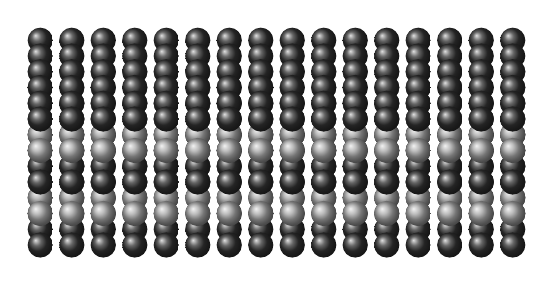
\begin{tikzpicture}[scale=0.4]
		\def\nuPi{3.1459265}
		\foreach \i in {15,14,...,0}{% This one doesn't matter
			\foreach \j in {5,4,...,0}{% This will crate a membrane
									% with the front lipids visible
			% top layer
			\pgfmathsetmacro{\dx}{0.5}% A random variance in the x coordinate
			\pgfmathsetmacro{\dy}{0.5}% A random variance in the y coordinate,    
			\shade[ball color=black!80] (\i+\dx,{0.5*\j+\dy+ 4} ) circle(0.4);
			\shade[ball color=gray!70] (\i+\dx,{0.5*\j+\dy+ 3}) circle(0.4);
			% bottom layer
			\pgfmathsetmacro{\dx}{0.5}
			\pgfmathsetmacro{\dy}{0.5}
			\shade[ball color=black!80] (\i+\dx,{0.5*\j+\dy+2}) circle(0.4);
			\shade[ball color=gray!70] (\i+\dx,{0.5*\j+\dy+1}) circle(0.4);
			\shade[ball color=black!80] (\i+\dx,{0.5*\j+\dy+0}) circle(0.4);
			}
		}
	\end{tikzpicture}
